\documentclass[10pt]{article}
\usepackage[margin=18mm]{geometry}
\usepackage[T1]{fontenc}
\usepackage{graphicx,booktabs,url}
\usepackage[colorlinks=true,urlcolor=blue]{hyperref}
\setlength{\parindent}{0pt}
\setlength{\parskip}{4pt}
\begin{document}\small
{\LARGE Native oracle and presentation components}\par
{\large 2026-10-18: audit items 4, 15, 16, 17}

\textbf{Status: partial against the original requests.} All fixtures are public
and synthetic. Complete four-presentation descent, measured solving degree,
production integration and full n83 relation solving remain open. Input
polynomial degree is different from F4 solving degree.

\textbf{Host:} shared Linux x86\_64, four-core CPU quota, 16GiB memory, L0.
No timing comparison or speedup is admitted. Frozen protocols, commands,
source/binary hashes, raw records, source snapshots and failures are retained.

\section*{Multiword n83 construction}
Modulus \texttt{0x800000000000000000095}; primitive 167th root
\texttt{0x76e02ca1a43987ce0230e}. C1 has 167 elements; C2 has 13,861 distinct
sums of two different roots, with every witness retained. The ONB has rank
83; both sets are Frobenius closed. All 334 generic-backend checks and
4096 full-width probes agreed; all probes were nonmembers. Generic replay
checked all 13,861 witnesses and Frobenius images, plus 167 root-order steps.
An altered witness was rejected with exit101; the original passed.

This component needs no exponential subgroup-log table. It does not
perform subgroup projection, useful-rank measurement or a full n83 solve.
Existing production cyclotomic code remains single-word.

\section*{Coordinate and complete addition strata}
Curve \texttt{icv1-f2m7-t13-616700dd}: K0, modulus 0x83, order 116.
The map $[X:Z]\mapsto[Z:X+Z]$ retains its pole and infinity; exact
polynomial-prefix bases are transported unchanged.
\begin{center}\begin{tabular}{rrrrrr}
\toprule
$(m,\ell)$&Lifted points&Pair checks&Tuple checks&Pole points&Distinct sums\\
\midrule
$(3,4)$&9&100&729&2&56\\
$(4,3)$&3&16&81&2&4\\
\bottomrule\end{tabular}\end{center}
Identity, inverse/two-torsion, doubling and generic checks passed. Every
tuple retained its sum. The ell=3 base has only three small-torsion points;
it supplies no effectiveness or yield evidence.
\begin{center}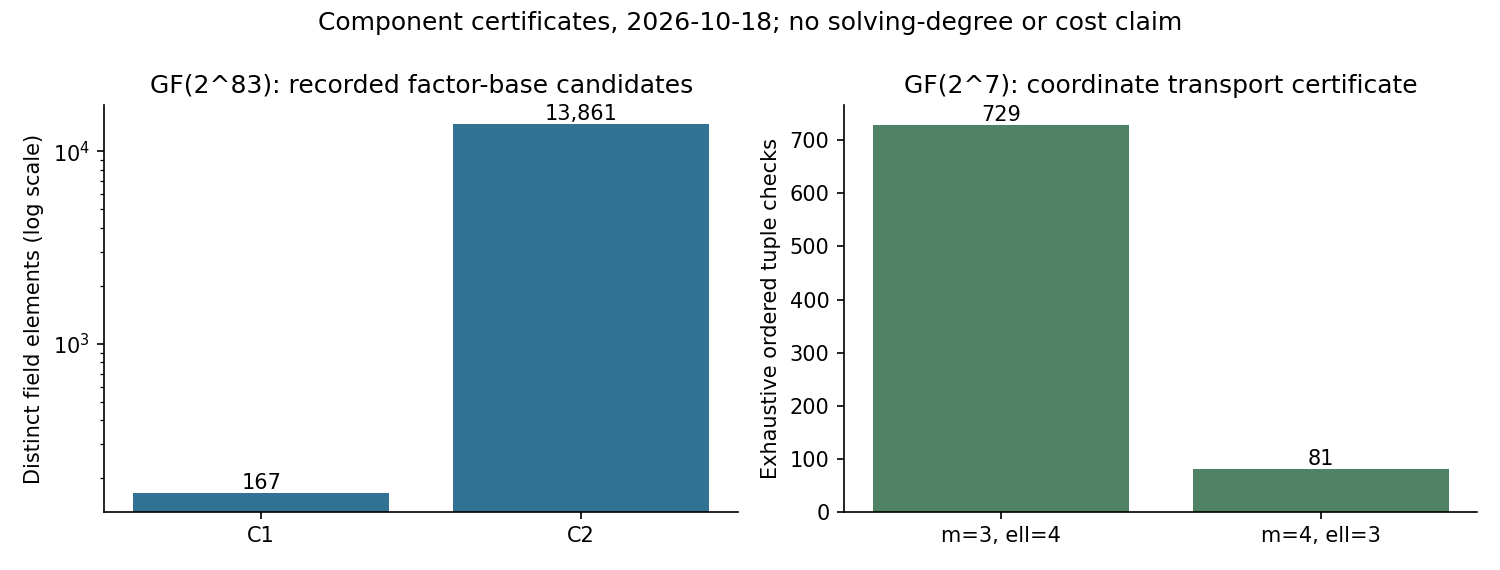
\includegraphics[width=.90\textwidth]{components.png}\end{center}

\textbf{Reproduction.} Study directory:
\path{research/ideas_execution_20261018/oracle_integration/}.
See \path{README.md}, \path{commands.txt}, \path{status.json}, the frozen
protocols and \path{runs/}. Native source:
\path{examples/ideas_oracle_components.rs} at repository root.

\newpage
\section*{Exact original equivariant panels}
All 24 step targets($n=7,11,13$,8 each) and 48 full-oracle targets
($n=5,7,11,13$,12 each) ran. Step tests equality of refutation and linear
consequences; oracle checks exact roots against independent brute enumeration.
\begin{center}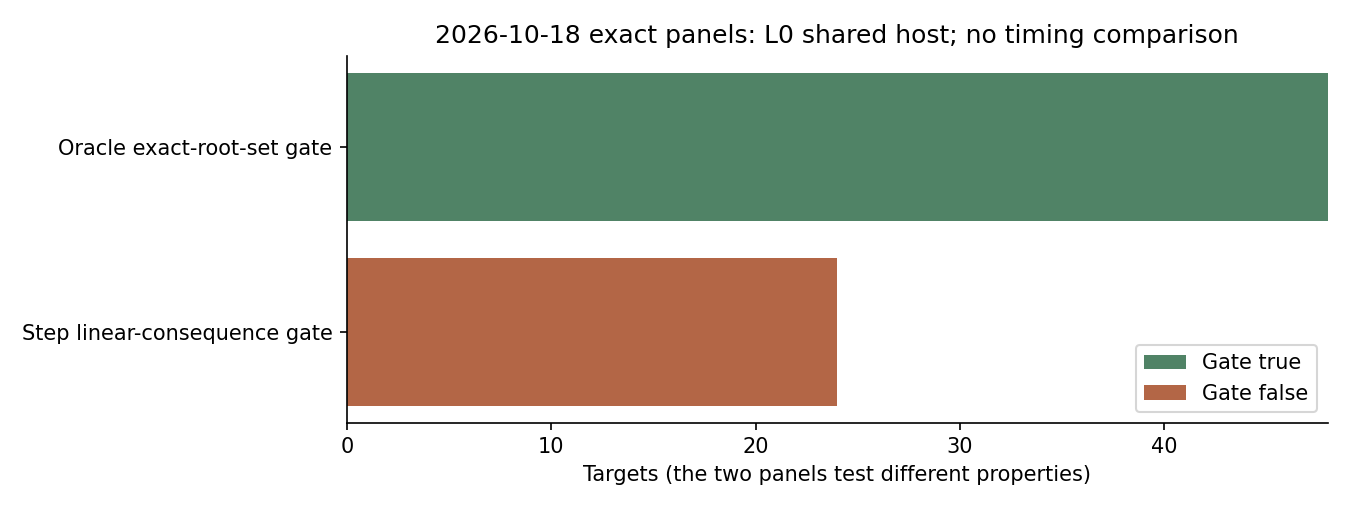
\includegraphics[width=.90\textwidth]{gates.png}\end{center}
The step replacement gate failed 24/24; containment held 24/24. The separate
full-oracle gate passed 48/48, including the repeated incumbent. Fixed-target
production lacks the barrel system's Frobenius symmetry. No invalid
production hook was installed.

\section*{Executed quadratic Boolean inputs}
\begin{center}\begin{tabular}{lrrrr}
\toprule
Input&Variables&Equations&Monomials&Input degree\\
\midrule
Generic addition(n7)&56&49&952&2\\
Doubling(n7)&42&42&580&2\\
C2 membership(n83)&1494&1494&159322&2\\
\bottomrule\end{tabular}\end{center}
Addition charts include nonzero-denominator inverse witnesses. Curve ANFs
agreed with independent membership on all 16,384 affine coordinate pairs.
Graph zero sets matched independent sums on all 8280 and 690 applicable
pair/output assignments over all 115 finite curve points. Exceptional
strata retain separate certificates.

The n83 input encodes $z_0^{167}=z_1^{167}=1$, $x=z_0+z_1$, $xw=1$ with
Frobenius linear wires and quadratic products. All 32 positives passed;
all 32 changed-x and 32 repeated-root controls were rejected. Complete
ANFs are retained; F4 on 1494 variables has not been run.
\begin{center}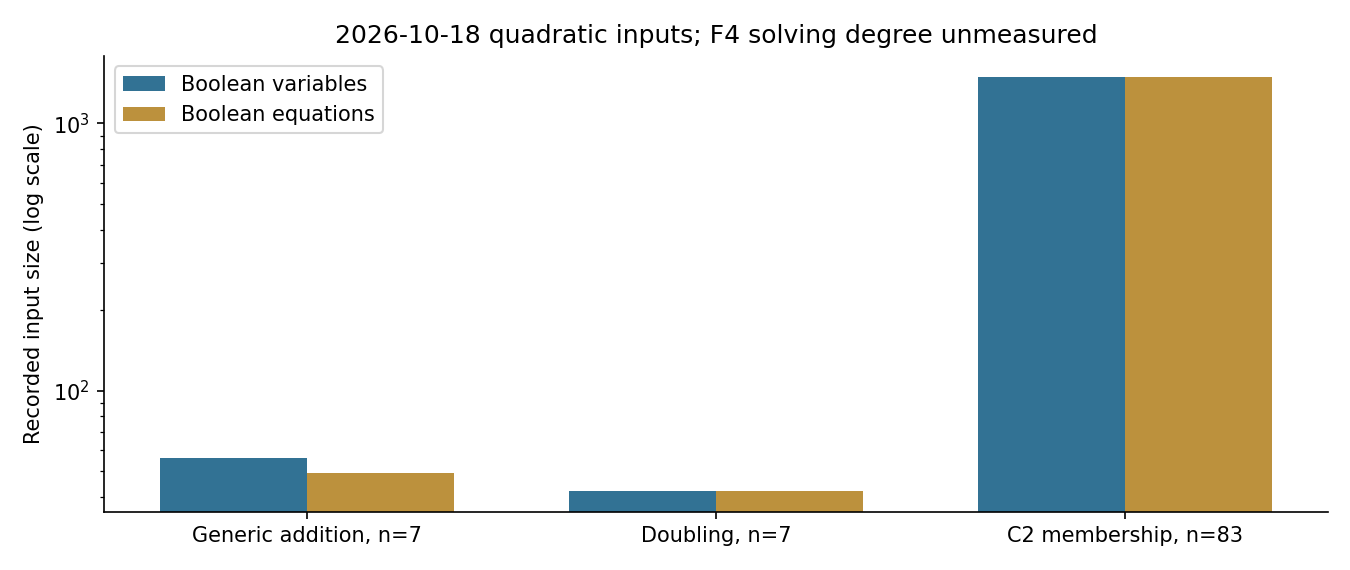
\includegraphics[width=.78\textwidth]{encodings.png}\end{center}
\textbf{Remaining original criteria:} Edwards/theta equations, complete same-base
four-presentation m-sum systems, measured D/Macaulay/solve costs, production
ecbench ablations, n83 subgroup/decomposition continuation and useful rank.
Root's n23 solver package is separate.

\newpage
\section*{Additional complete factorial attempts}
The unchanged seven-arm spec first ran under the owner's published native
release v0.1.2538. Its source commit is:
\begin{center}\texttt{b1bf5b8935f68257dfdd3fc542cb2fef41db741c}\end{center}
The archive passed publisher checksums. Session \texttt{ECBS1h328da50bcef9}
completed all 224 attempts: 152 verified, 72 exhausted. A/A matched 32/32
workloads, including failures. Audit passed 152 verified-run replays with
zero problems; exhausted records were retained but not replayed. The prior
36-record D4 session also audited cleanly with 12 exact replays.
\begin{center}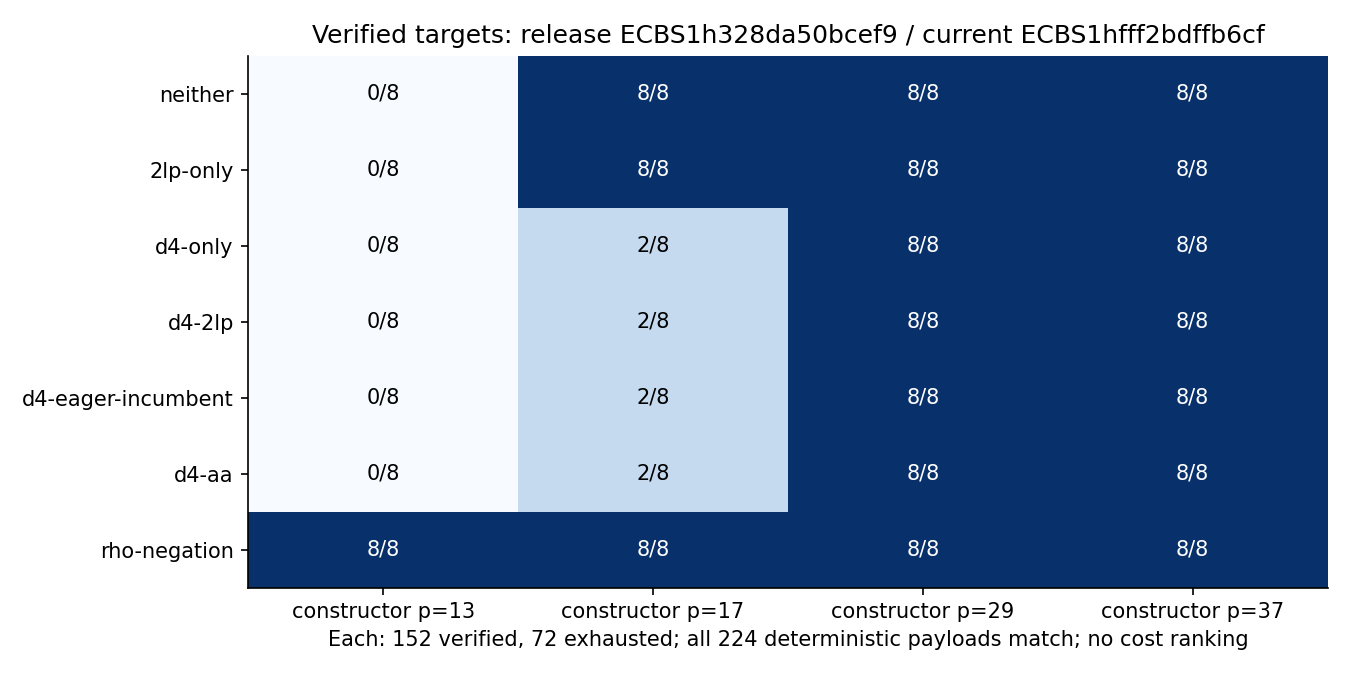
\includegraphics[width=.90\textwidth]{factorial-outcomes.png}\end{center}

\textbf{Admission limits.} Four constructor curves await registration. IC
charges include a historical algebraic-solve model and unpriced stand-in
oracle. Native comparisons mark the panel incomplete and diagnostic. The
0/0.1/1 GAE band covers every declared unpriced counter on every arm,
including rho; missing counters are exposed. Unknown non-emitted
bookkeeping remains outside that band. No complete-cost ranking or citable
curve-specific conclusion is admitted. Native output permits wall values
under its L0 spec; this report rejects that timing admission.

\textbf{Current-build repair.} The CLI initially failed because of a missing
\texttt{fbm} import. Root authorized the minimal import; current CLI test
and release build passed. Current session \texttt{ECBS1hfff2bdffb6cf} repeated
all 224 attempts with the same 152 verified/72 exhausted outcomes, 32/32 A/A
matches, and 152 verified-run replays. An exact native comparison matched
all 224 deterministic target/outcome/cost/counter/detail payloads across
the two binaries, including all 72 exhausted runs. Timings/source labels
were excluded. The release session was not overwritten.

\textbf{Prior evidence retained.} D4+2LP had already measured 1.025
[1.016,1.037] on 24 held-out curves; round2 eager D4 measured 0.9792
[0.9725,0.9855] on 27. The trace filter rejected 0/29,624 subgroup targets.
Free relations are already production default. These are prior results.

\textbf{Validation.} Component Cargo tests passed 3/3; release build passed.
The analysis example built and its zero-test target passed. Parent's full
library suite reported 4378 passed, 4 failed, 117 ignored before separate
baseline repair. Those files were not edited here; no full-suite pass is claimed.

\textbf{Sources.} Study \path{commands.txt} and \path{runs/}; prior studies
\path{research/ic_improve_20261014/01-d4-2lp/},
\path{research/ic_improve_20261015/04-d4-2lp-fix/},
\path{research/ic_improve_20261014/03-tracezero-freerel/}, and
\path{research/ic_improve_20261015/02-freerel-production/}.
\end{document}
